\section{Обзор существующих решений}
\label{sec:Chapter2} \index{Chapter2}

Существует ряд работ, в которых решается задача извлечения иерархической структуры из документов разных видов.
В работах предлагается то представление, к которому приводятся обрабатываемые документы.

Основополагающей работой в данном направлении является статья о представлении структуры документа~\cite{dori1997representation}.
Несмотря на большое разнообразие видов логической структуры, в этой работе
предлагается <<общая логическая структура>>, в которой любой документ представляется в виде дерева.
Листьями такого дерева являются символы, которые затем объединяются в слова,
слова в предложения, предложения в параграфы, и т.д. (рисунок~\ref{fig:dori1997representation}).
\begin{figure}[h]
        \begin{center}
        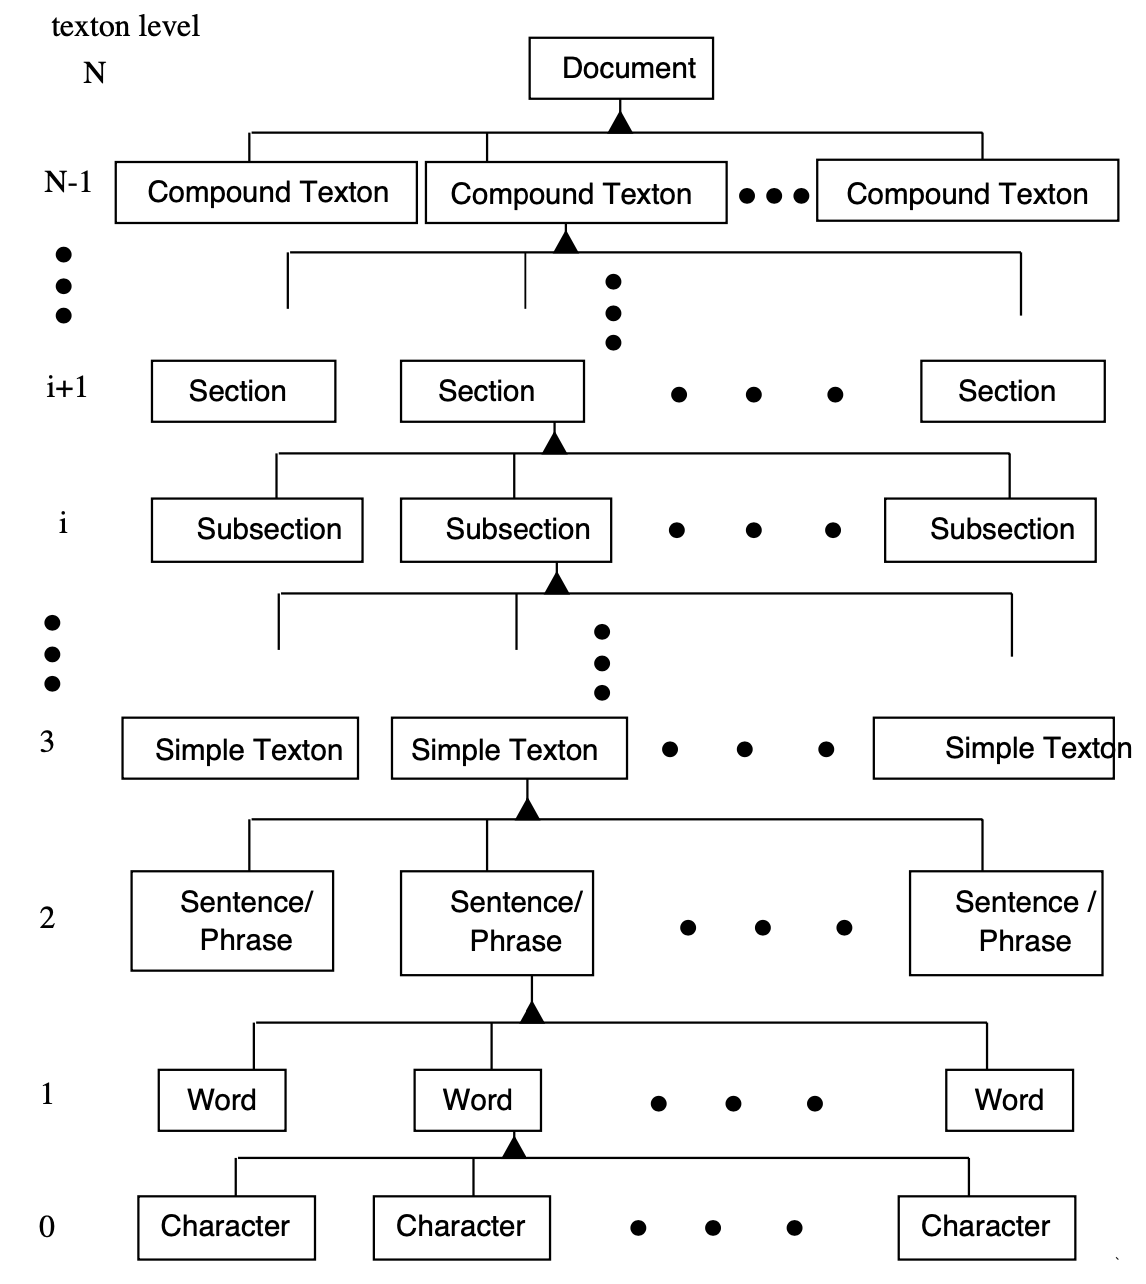
\includegraphics[width=0.6\textwidth]{img/dori1997representation}
        \caption{Предлагаемая в~\cite{dori1997representation} общая логическая структура документа в виде дерева}
        \label{fig:dori1997representation}
        \end{center}
\end{figure}
\todo[inline]{Дописать про метод}

В большая части существующих работ рассмотрение документов ограничивается определённой предметной областью,
так как в этом случае при извлечении структуры можно опираться на семантику конкретной группы документов.
\todo[inline]{Примеры и ссылки}